\chapter{WebSocket Messaging System}
\label{chapter:websocketMessagingSystem}

This chapter provides information regarding the requirements and tooling for a WebSocket based messaging system. Afterwards the design and implementation of the system itself is introduced before benchmarking results and ideas for possible improvements are presented.

\section{Requirements}

The WebSocket messaging system allows a web chat client to communicate with a backend service using the WebSocket protocol rather than polling or long-polling. The system should be an improvement over HTTP-based implementations as it causes less network load and information can be updated instantly when available. The system must be capable of serving multiple concurrent clients while guaranteeing reliable message delivery.
\\ \\
The development of the WebSocket messaging system takes place while a HTTP-based implementation is in production. Thus it must be able to co-exist with the current implementation and be functional with the same backend setup. The components of the system should consist of modular and exchangeable microservices so that individual parts of the system can be scaled independently. Finally the system should be able to run on a Linux-based infrastructure.

\section{Tools}

The following tools were used to implement the WebSocket messaging system. They are by far the only tools available for the development of this kind of system but were deemed suitable based on accessibility, documentation and community backing.

\subsection{Node.js}

Node.js is an open source, cross-platform runtime environment for server-side and networking applications written in Javascript. It provides an event-driven architecture and a non-blocking I/O API optimized for throughput and scalability. Node.js operates on a single thread, making it possible to support multiple concurrent connections without incurring the cost of context-switching. Those properties make Node.js specially suitable for real-time and high concurrent applications. The WebSocket messaging system was implemented using JavaScript and two different Node.js versions were used to benchmark the system.

\subsection{ZeroMQ}

ZeroMQ is a messaging library for for distributed applications with an asynchronous I/O model. It offers the possibility of various messaging patterns such as request-reply, publish-subscribe and push-pull. One of the main advantage of ZeroMQ for application developers is that it manages various low-level networking considerations such as buffering and reconnection. That can lead to a more simple application development process and more robust distributed systems. ZeroMQ was used to send data between different components of the WebSocket messaging system using push sockets.

\subsection{Nginx}

Nginx is an open-source reverse proxy server with support for various protocols. It can also work as a load balancer, HTTP cache and web server. It uses an asynchronous event-driven approach for handling requests which make it capable of high concurrency and low memory footprint. Nginx was used as a reverse proxy server for the WebSocket messaging system that listens to ports 80 and 443 for HTTP and HTTPS traffic.

\section{Design and Implementation}

The WebSocket messaging system is designed to allow the clients and server to exchange data over a persistent WebSocket connection while data is served from the backend over a HTTP-based API. One challenge related to that kind of data exchange and the decision to use Node.js to implement the system is the single threaded nature of Node.js. To work around that aspect the the cluster module of Node.js will be used that makes it possible to take advantage of multi-core systems by making it possible to launch a cluster of processes. Another design decision is to keep the system in loosely coupled and fine grained components in accordance with the microservices ideology. This kind of architecture would make it possible to scale individual parts of the system for performance enhancement and distribute the system strategically, when put into production, to possibly reduce latency. Figure~\ref{fig:webSocketMessagingSystem} shows the structure of the WebSocket messaging system and the relationship between different components which are explained in the following sections.

\begin{figure}[h!]
	\centering
	\label{fig:webSocketMessagingSystem}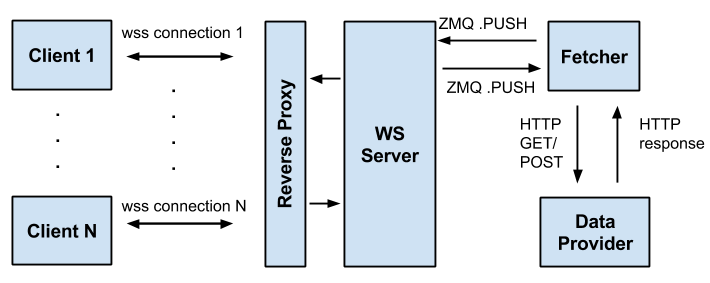
\includegraphics[width=1\textwidth]{images/websocketMessagingSystem}
	\caption{Structure of the WebSocket messaging system}
\end{figure}

\subsection{Clients}

A client opens up a connection with the WebSocket server and makes a request for specific keys. In the case of a chat application these keys would most likely be conversation identifiers that are kept in a persistent storage on the backend side. Different clients request different keys based on the conversations they are a part of and thus subscribed to. In the case of the WebSocket messaging system the client is simply a viewer for data randomly generated by the data provider. The system is designed to support multiple concurrent connections between clients and the WebSocket server.

\subsection{Reverse Proxy}

The reverse proxy is used as a tunnel between the clients to the WebSocket server and provides an encrypted connection with Transport Layer Security. The load balancing capabilities of Nginx make it possible to scale individual parts of the system. This approach makes it possible to scale the system horizontally when bottlenecks have been identified for better infrastructure utilization.


\subsection{WebSocket Server}

The WebSocket server listens on a specific port and establishes a WebSocket connection upon request. Further connection management is dependent on the WebSocket implementation used by the server. The Node.js WebSocket implementation used in the system is called ws\footnote{\url{https://github.com/websockets/ws}} and adds no extra functionality to the WebSocket API and protocol specifications. The aim of the project is to stay up to date with RFC 6455 while providing a simple and fast implementation of WebSocket.
\\ \\
After a WebSocket connection had been established the server is responsible for returning data associated with the key requested by a client. Either the server has the data in memory or it must request it from the fetcher using a push socket over a TCP connection using the ZeroMQ library. The communication with the fetcher goes through a ZeroMQ client is needed in able to use the binary protocol of the library.

\subsection{Fetcher}

The fetcher maintains a queue of requests made by the WebSocket server and manages a cluster of worker processes that handle the HTTP requests to the data provider. This technique makes it possible to have separate processes share the same server port and take an advantage of the available cores on the host machine. A master process listens on a port, accepts new connections and distributes them to available worker processes using a round-robin scheduling algorithm \cite{nodeCluster}. The worker processes are spawned such that they can communicate with the master process via IPC and are capable of passing server handles back and forth. The master process is then responsible for managing the worker process to avoid overloading and load-balance requests from the WebSocket server to different workers.
\\ \\
The clustering approach allows the WebSocket messaging system to improve throughput and resource utilization when managing production workload by taking advantage of multicore processors despite the single threaded nature of Node.js. Another advantage of this approach compared to communication patterns like polling and long-polling is that the fetcher and the data provider and be places geographically close to each other which can reduced latency.

\begin{figure}[h!]
	\centering
	\label{fig:webSocketMessagingSystem}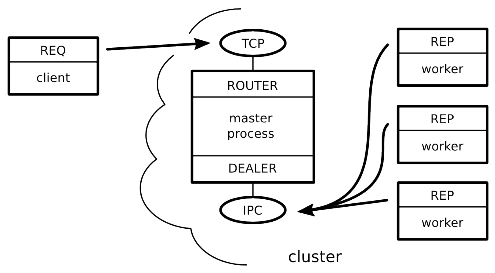
\includegraphics[width=0.9\textwidth]{images/poolOfWorkers}
	\caption{A Node.js cluster that routes requests to a pool of workers \cite{judd2008node}}
\end{figure}

\subsection{Data Provider}

The data provider serves JSON or random text and binary data over a HTTP-based API. In this implementation the data provider does not provide any meaningful data but has the purpose of simulating the data source that the WebSocket messaging system is intended to eventually use.

\section{Benchmarking}

The purpose of the benchmarking tests was to figure out how many concurrent clients the messaging system could handle without dropping connections. The results can be used as a basis for capacity planning of a WebSocket-based infrastructure or used to analyse the WebSocket messaging system for further development.
\\ \\
The load test was implemented so that a new client connects to the WebSocket server every two seconds and requests a 130 KB JSON file every second. The benchmarking was done for two different instance types, one with 4GB RAM  and 2 CPUs and another one with 8GB RAM and 4 CPUs. Both instances had SSD drives and were located in a datacenter in Frankfurt with the clients that made request located in Iceland. Version 0.10.38 of Node.js (the minor version provided in repositories of most common Linux distros) was used to run all the components of the system that were deployed on a Ubuntu 14.04.2 LTS OS with a 3.13.0-52 Linux kernel. The Nodetime\footnote{\url{https://nodetime.com/}} application monitoring and analytics service was for performance measurement in addition to the \texttt{iptraf} Unix tool for network monitoring.
\\ \\
The metrics of the benchmarking test were: Available memory, CPU time, V8 heap used and full garbage collections while the WebSocket messaging system was able to cope with increasing number of concurrent client connections. The results can be seen in the graphs below.

\begin{figure}[h!]
	\centering
	\subfigure[4GB RAM / 2 CPUs]{\label{fig:freeMemory-2cpus}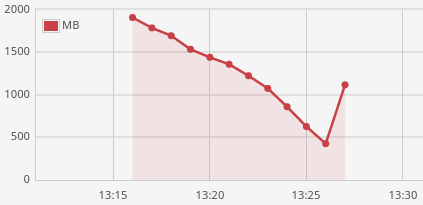
\includegraphics[width=0.45\textwidth]{images/freeMemory-2cpus}} \hfill
	\subfigure[8GB RAM / 4 CPUs]{\label{fig:freeMemory-4cpus}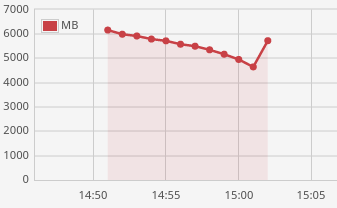
\includegraphics[width=0.45\textwidth]{images/freeMemory-4cpus}}
	\caption{Free memory (MB)}
\end{figure}

\begin{figure}[h!]
	\centering
	\subfigure[4GB RAM / 2 CPUs]{\label{fig:cpuTime-2cpus}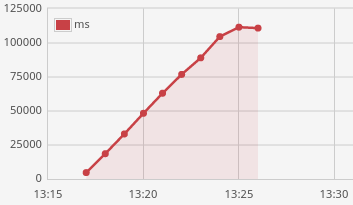
\includegraphics[width=0.45\textwidth]{images/cpuTime-2cpus}} \hfill
	\subfigure[8GB RAM / 4 CPUs]{\label{fig:cpuTime-4cpus}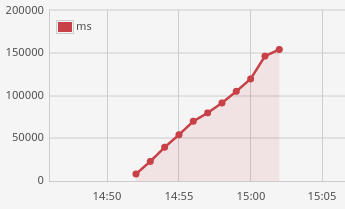
\includegraphics[width=0.45\textwidth]{images/cpuTime-4cpus}}
	\caption{CPU time  (ms)}
\end{figure}

\begin{figure}[h!]
	\centering
	\subfigure[4GB RAM / 2 CPUs]{\label{fig:v8heapUsed-2cpus}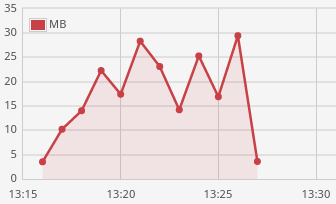
\includegraphics[width=0.45\textwidth]{images/v8heapUsed-2cpus}} \hfill
	\subfigure[8GB RAM / 4 CPUs]{\label{fig:v8heapUsed-4cpus}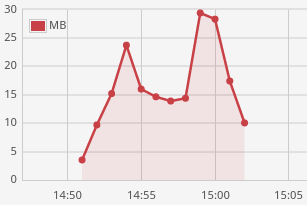
\includegraphics[width=0.45\textwidth]{images/v8heapUsed-4cpus}}
	\caption{V8 heap used (MB)}
\end{figure}

\begin{figure}[h!]
	\centering
	\subfigure[4GB RAM / 2 CPUs]{\label{fig:fullGcs-2cpus}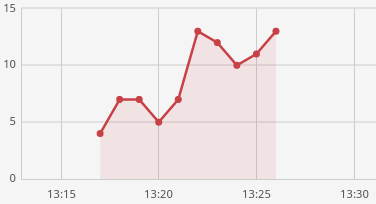
\includegraphics[width=0.45\textwidth]{images/fullGcs-2cpus}} \hfill
	\subfigure[8GB RAM / 4 CPUs]{\label{fig:fullGcs-4cpus}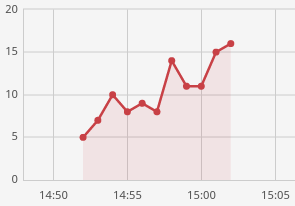
\includegraphics[width=0.45\textwidth]{images/fullGcs-4cpus}}
	\caption{Full garbage collections per minute}
\end{figure}

\begin{table}[h!]
\begin{tabular}{lll}
\hline
	& \textbf{4GB RAM / 2 CPUs}	&	\textbf{8GB RAM / 4 CPUs} \\ \hline
\textbf{Concurrent connections}	& 304	& 333 \\
\textbf{Data sent (MB/sec)}	& 46,34	& 47,17 \\
\hline                         
\end{tabular}
\caption{Number of concurrent connections and data rate}
\label{table:connectionsDatarate}
\end{table}

\section{Possible Improvements}

Use a different version of Node (a newer V8 engine might do something..)


